\documentclass[12pt]{article}
\usepackage{cite}
\usepackage[affil-it]{authblk}
\usepackage{textcomp}
\usepackage[margin=1.0in]{geometry}
\usepackage[sort&compress,numbers]{natbib}
\usepackage{setspace}
\usepackage{indentfirst}
\usepackage{compactbib}
\usepackage{setspace}
\usepackage{authblk}
\usepackage{mathdots}
\usepackage[hidelinks]{hyperref}
\usepackage{color}
\usepackage{gensymb}
\usepackage{amsmath}
\usepackage{amssymb}
\usepackage{amscd}
\usepackage[pdftex]{graphicx}
\usepackage{nicefrac}
\usepackage[np,autolanguage]{numprint}
\usepackage{longtable}
\usepackage{bm}
\usepackage{subfigure}
\usepackage{float}
\usepackage{morefloats}
\usepackage{chngcntr}
\usepackage{braket}
\usepackage{mhchem}
\usepackage{enumitem}
\linespread{1.5}
\newcommand{\be}{\begin{equation}}
\newcommand{\ee}{\end{equation}}
\setlength{\LTcapwidth}{\textwidth}
%==============================================================================%
%                             Title Information                                %
%==============================================================================%
\title{Diatomic Potential Notes}
\date{\today}
\author{Alan Robledo}
%==============================================================================%

\begin{document}
\maketitle
\section{Theory}
\subsection{Rovibrational motion in diatomic molecules}
The relative motion of two nuclei can be described in terms of the motion of a fictitious particle with mass $\mu$ moving in an effective potential $V_{eff}$, resulting in a 3 dimensional problem (excluding center-of-mass motion).\cite{mitnotes}\cite{zhang} The fictitious mass is denoted as a reduced mass, which is defined as,
\be
  \mu = \frac{m_1m_2}{m_1+m_2} .
\ee
This 3 dimensional Hamiltonian can be written in spherical coordinates as,
\be
    \hat{H} = \frac{\textbf{p}^2}{2\mu} + V(r) = -\frac{\hbar^2}{2\mu} \frac{1}{r} \frac{\partial^2}{\partial r^2} r + \frac{\textbf{L}^2}{2\mu r^2} + V(r)
\ee
where $\textbf{L}^2$ is the angular momentum operator that is defined as,
\be
    \textbf{L}^2 = -\frac{\hbar^2}{\sin^2\theta} \left(\sin\theta \frac{\partial}{\partial \theta} \sin\theta \frac{\partial}{\partial \theta} + \frac{\partial^2}{\partial^2 \phi^2} \right) .
\ee
One method for solving this equation is by considering that the full wavefunction $\Psi(r,\theta,\phi)$ can be written as a product of a radial function $R(r)$ and an angular function $Y(\theta,\phi)$.\cite{mitnotes} Plugging this into the Schr\"odinger equation with the Hamiltonian described above gives us,
\be
    \left[ -\frac{\hbar^2}{2\mu} \frac{1}{r} \frac{\partial^2}{\partial r^2} r + \frac{\textbf{L}^2}{2\mu r^2} + V(r) \right] R(r) Y(\theta,\phi) = ER(r)Y(\theta,\phi)
\ee
We know from solving the hydrogen atom that the angular function $Y(\theta,\phi)$ is an eigenstate of $\textbf{L}^2$.
\be
    \textbf{L}^2 Y(\theta,\phi) = \hbar^2 \ell(\ell+1)Y(\theta,\phi)
\ee
Using this fact and seeing that $Y(\theta,\phi)$ can be cancelled out lets us write the Schr\"odinger equation as,
\be
    -\frac{\hbar^2}{2\mu} \frac{1}{r} \frac{\partial^2}{\partial r^2} rR(r) + \frac{\hbar^2 \ell(\ell+1)}{2\mu r^2}R(r) + V(r) R(r) = ER(r)
\ee
Multiplying both sides of the equation by r gives,
\be
    -\frac{\hbar^2}{2\mu} \frac{\partial^2}{\partial r^2} rR(r) + \frac{\hbar^2 \ell(\ell+1)}{2\mu r^2}r R(r) + V(r) r R(r) = E r R(r)
\ee
which suggests introducing a modified radial function u(r) such that
\be
    R(r) = \frac{u(r)}{r} .
\ee
This leaves us with what looks like a one dimensional Schr\"odinger equation,
\be
    -\frac{\hbar^2}{2\mu} \frac{\partial^2}{\partial r^2} u(r) + V_{eff} u(r) = E u(r)
\ee
where the effective potential $V_{eff}$ as described in the beginning is,
\be
    V_{eff} = \frac{\hbar^2 \ell(\ell+1)}{2\mu r^2} + V(r) .
\ee
V(r) is a potential energy that describes the interaction between the two nuclei. The goal of this project is to numerically compute the energies of any diatomic molecule of our choosing using a basis set method when $\ell = 0$. $V(r)$ can be generated using any computational chemistry software package, which leads to us choosing a basis set to carry out the calculations.

\subsection{Particle in a box basis}
Using the particle in a box eigenfunctions as our basis, we start by defining,
\be
    \ket{\phi} = \sum_n C_n \sqrt{ \frac{2}{a}} \sin \left(\frac{n \pi x}{a} \right)
\ee
where $C_n$ are epansion coefficients.\cite{zhang}
Since our problem consists of two atoms at some points $r_1$ and $r_2$, separated by some distance r, we can incorporate this information into our basis definition by defining $x = r - r_1$ and $a = r_2 - r_1$ (see Figure 1).
\begin{figure}[H]
    \centering
    % height adjusts the size of the photo.
    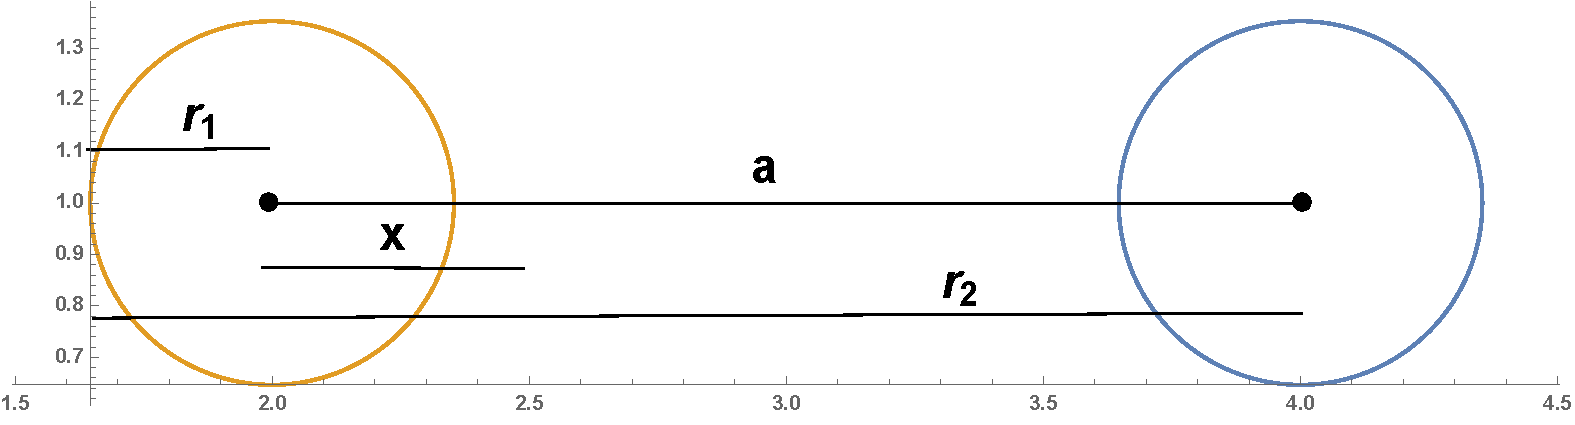
\includegraphics[height=1.8in]{figures/graphic.pdf}
    \caption{An example of two nuclei, one nuclei at $r = r_1 = 2.0$ and another at $r = r_2 = 4.0$. The distance between the two nuclei is denoted as a (also known as the length of the box), and the coordinate x is shown to be at $0.5$. This figure is an example of how two nuclei can be related to a particle in a box.}
\end{figure}
Therefore, $\ket{\phi}$ is defined as,
\be
    \ket{\phi} = \sum_n C_n \sqrt{ \frac{2}{r_2-r_1}} \sin \left(\frac{n \pi (r - r_1)}{r_2 - r_1} \right)
\ee
Since the set of particle in a box eigenfunctions form an orthonormal set, the overlap matrix elements would simply evaluate to kronecker deltas, i.e. $S_{ij} = \delta_{ij}$.
Elements of the Hamiltonian matrix are computed as,
\be
\begin{split}
    \braket{\phi_m|\hat{H}|\phi_n} &= \braket{\phi_m|\hat{T} + \hat{V}|\phi_n}\\
    &= \braket{\phi_m|\hat{T}|\phi_n} + \braket{\phi_m|\hat{V}|\phi_n} \\
\end{split}
\ee
The Hamiltonian for our system in atomic units is defined as,
\be
    \hat{H} = \hat{T} + \hat{V} = \frac{-1}{2\mu} \frac{\partial^2}{\partial r^2} + \frac{\ell(\ell+1)}{2\mu r^2} + V(r)
\ee
The matrix elements of the kinetic energy are:
\be
\begin{split}
    \braket{\phi_m|\hat{T}|\phi_n} &= \int_{r_1}^{r_2} \phi_m(r) \hat{T} \phi_n(r) dr \\
    &= \int_{r_1}^{r_2} \sqrt{\frac{2}{r_2 - r_1}} \sin \left( \frac{m \pi (r - r_1)}{r_2 - r_1} \right) \hat{T} \sqrt{\frac{2}{r_2 - r_1}} \sin \left( \frac{n \pi (r - r_1)}{r_2 - r_1} \right) dr \\
    &= \int_{r_1}^{r_2} \frac{2}{r_2 - r_1} \sin \left( \frac{m \pi (r - r_1)}{r_2 - r_1} \right) \left( \frac{-1}{2 \mu} \frac{d^2}{dr^2} \right) \sin \left( \frac{n \pi (r - r_1)}{r_2 - r_1} \right) dr \\
\end{split}
\ee
The inner derivative is trivial.
\be
\begin{split}
    \frac{d^2}{dr^2} \left( \sin \left( \frac{n \pi (r - r_1)}{r_2 - r_1} \right) \right) &= \frac{d}{dr} \left( \frac{n \pi}{r_2 - r_1} \cos \left( \frac{n \pi (r - r_1)}{r_2 - r_1} \right) \right)\\
    &= \frac{-(n \pi)^2}{(r_2 - r_1)^2} \sin \left( \frac{n \pi (r - r_1)}{r_2 - r_1} \right) \\
\end{split}
\ee
Therefore, the kinetic energy in matrix form is written as,
\be
\begin{split}
    \braket{\phi_m|\hat{T}|\phi_n} &= \frac{(n\pi)^2}{2 \mu(r_2 - r_1)^2} \int_{r_1}^{r_2} \frac{2}{r_2 - r_1} \sin \left( \frac{m \pi (r - r_1)}{r_2 - r_1} \right) \sin \left( \frac{n \pi (r - r_1)}{r_2 - r_1} \right) dr \\
    &= \frac{(n \pi)^2}{2 \mu (r_2 - r_1)^2} \delta_{mn}\\
\end{split}
\ee
The matrix elements of the potential energy are:
\be
\begin{split}
    \braket{\phi_m|\hat{V}|\phi_n} &= \int_{r_1}^{r_2} \phi_m(r) \hat{V} \phi_n(r) dr \\
    &= \int_{r_1}^{r_2} \sqrt{\frac{2}{r_2 - r_1}} \sin \left( \frac{m \pi (r - r_1)}{r_2 - r_1} \right) \hat{V} \sqrt{\frac{2}{r_2 - r_1}} \sin \left( \frac{n \pi (r - r_1)}{r_2 - r_1} \right) dr \\
    &= \frac{2}{r_2 - r_1} \int_{r_1}^{r_2} \left( \frac{\ell(\ell+1)}{2\mu r^2} + V(r) \right) \sin \left( \frac{m \pi (r - r_1)}{r_2 - r_1} \right) \sin \left( \frac{n \pi (r - r_1)}{r_2 - r_1} \right) dr \\
\end{split}
\ee

Eigenvalues are first found by solving the secular equation,
\be
    |\textbf{H} - E \textbf{I}| = 0
\ee
for E, which is an N order polynomial where N is determined by the user. And the eigenvectors are found by solving the eigenvalue equation,
\be
    (\textbf{H} - E \textbf{I}) \ket{a_i} = \ket{0}
\ee
for $\ket{a_i}$ where $\ket{0}$ is a vector of zeros. The eigenvector for each eigenvalue contains the expansion coefficients $c_n$ for the expansion of an eigenstate in terms of the basis functions. However, the program returns the eigenvectors as a matrix where the ith column represents the ith eigenvector. Therefore, the set of eigenvectors will be denoted as a matrix with elements $a_{mn}$ which become the expansion coefficients for the expansion of the eigenstate in terms of the basis states.
\be
    \ket{\phi_n} = \sum_{m = 1}^{N} a_{mn} \sqrt{ \frac{2}{r_2-r_1}} \sin \left(\frac{n \pi (r - r_1)}{r_2 - r_1} \right)
\ee

\bibliography{mybib}
\bibliographystyle{unsrt}

\end{document}
